\subsection{Active Armrest}
\label{ch:prot_armrest}
\begin{minipage}{\linewidth}
\centering
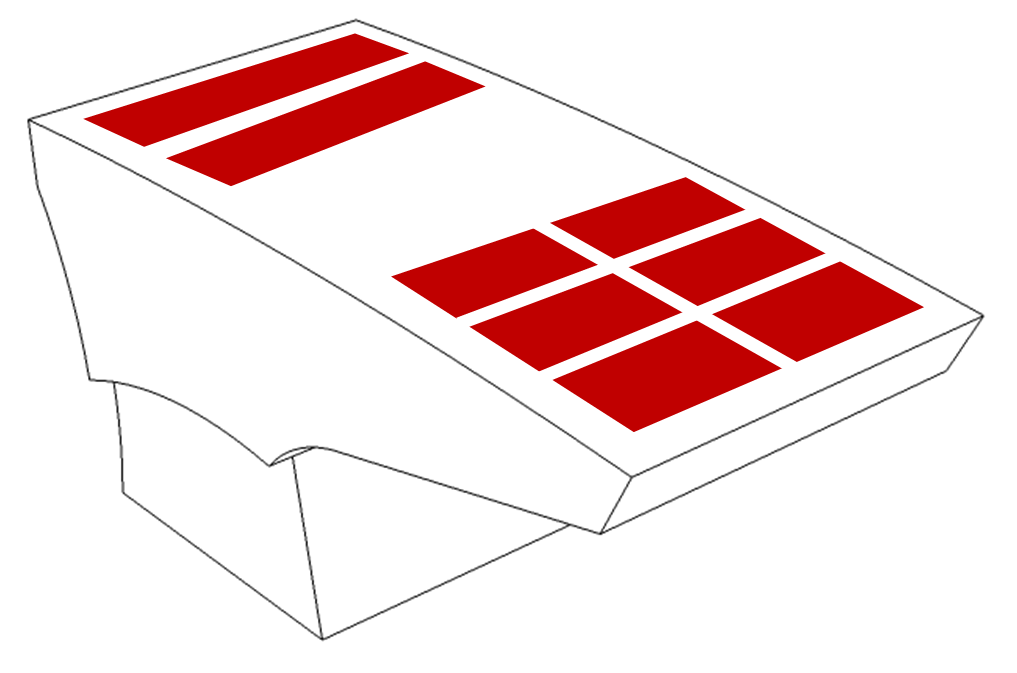
\includegraphics[width=0.4\textwidth]{images/active_armrest}
\captionof{figure}{Active armrest sketch - six electrodes for finger gesture detection in front, two for arm detection in back}
\label{fig:armrest_sketch}
\end{minipage}

Touch screens are by now also a trend in vehicles, with touch screens and touch pads becoming more common. The Tesla Model S provides a large area touch screen that completely replaces conventional button-based interfaces.  However, touchscreens have been identified as potentially distracting for the driver \cite{rumelin2013make}. Our idea was to create a gesture input device based on capacitive proximity sensors, and unobtrusively integrate it into the car interior. In this project I was collaborating with students Sönke Schmidt and Stephan Neumann \cite{braun2013ActiveArmrest}. A suitable area for creating an interactive zone is the armrest, as it is the intended resting position in the first place. However, this creates an additional challenge. As the majority of interactions between arm and armrest are not intended to control aspects of the car system, we need concepts to infer the intention of the driver to interact with the car. The method has been described previously in Section \ref{ch:proc_hetero}. A sketch of this concept is shown in Figure \ref{fig:armrest_sketch}. To test the validity of the invisible interactive areas and the two interaction concepts, we have created the Active Armrest, a prototype comprised of an aftermarket armrest with an integrated heterogeneous array of eight capacitive proximity sensors - two using large electrodes for detecting arm proximity and orientation and six using small electrodes to create an interaction area in front of the armrest. The system uses the classification method described in Section \ref{ch:proc_hetero}.

\begin{minipage}{\linewidth}
\centering
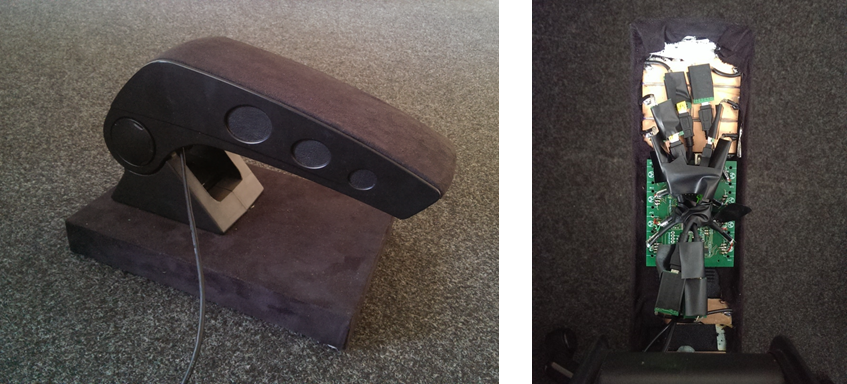
\includegraphics[width=0.8\textwidth]{images/armrest_proto}
\captionof{figure}{Active Armrest prototype, left - outside view, right - detail view of electronics \cite{braun2013ActiveArmrest}.}
\label{fig:armrest_proto}
\end{minipage}

In order to evaluate the Active Armrest we have built the prototype shown in Figure \ref{fig:armrest_dataproc}. An aftermarket armrest was equipped with an OpenCapSense toolkit. The kit had to be modified due to the constrained interior and uses fixed wiring instead of USB connection. The demonstration application is based on the SenseKit debug software supplied with the toolkit. As of now there is a simple USB connection to a nearby PC. The gesture recognition framework was implemented in Java using the WEKA machine learning framework for SVM classification. A car interior demonstration application was created using Java and the Swing framework and mimics typical menu systems found on a touch screen.

\begin{minipage}{\linewidth}
\centering
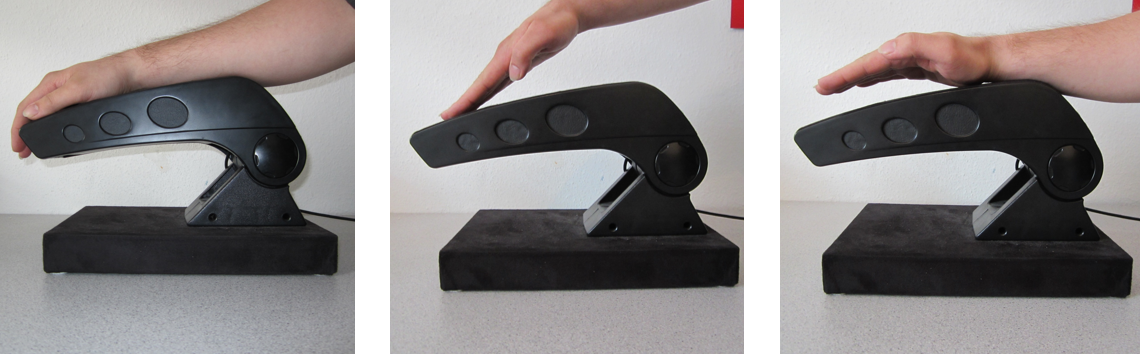
\includegraphics[width=0.8\textwidth]{images/armrest_postures}
\captionof{figure}{Postures of limbs on armrest - resting position (left),  arm raised position (middle), hand raised position (right) \cite{braun2013ActiveArmrest}.}
\label{fig:armrest_postures}
\end{minipage}

In Figure \ref{fig:armrest_postures} we can see the three different positions arm and hand can have on the armrest. On the left arm and hand are in resting position with both close to the surface. The middle image shows the arm raised position and fingers touching the front of the armrest. The right picture shows the arm resting on the back and the hand in proximity of the front area. The system is able to distinguish between the three different positions using the methods presented in Section \ref{ch:proc_hetero}. A set of four different gestures has been defined for both interaction methods. The number is sufficient to control the user interface that was developed and supports both navigation and selection. The type of gestures has been defined after looking at previous research into touch and hand gestures \cite{bragdon2011experimental, wachs2011vision}. For the touch interaction left and right swipes performed with either one or multiple fingers are supported. Regarding the free-air interaction we are using left and right swipes, as well as planar circles either clockwise or counter-clockwise.

\begin{minipage}{\linewidth}
\centering
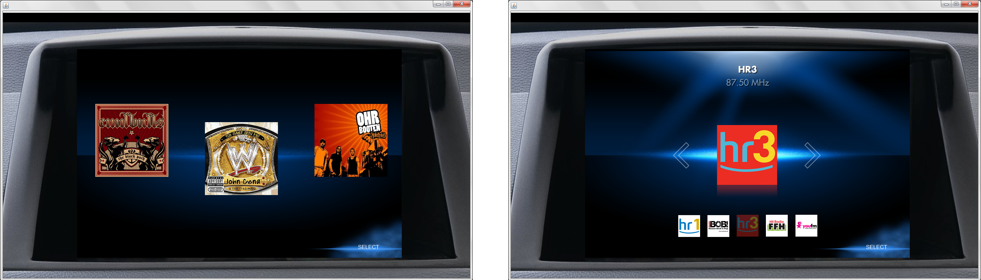
\includegraphics[width=0.8\textwidth]{images/armrest_demo_app}
\captionof{figure}{Active Armrest demo software, left - finger tracker, right - OSM based navigation application \cite{braun2013ActiveArmrest}}
\label{fig:armrest_demo_app}
\end{minipage}

Figure \ref{fig:armrest_demo_app} shows two screenshots of the created demonstration application. It allows to control radio stations, selecting different audio files and looking at images. It is controlled using the gesture sets explained above. The applications use a Next/Previous pattern for navigation within a UI level and Select/Back gestures to switch between the different levels of the UI.

\subsubsection{Evaluation}
\begin{minipage}{\linewidth}
\centering
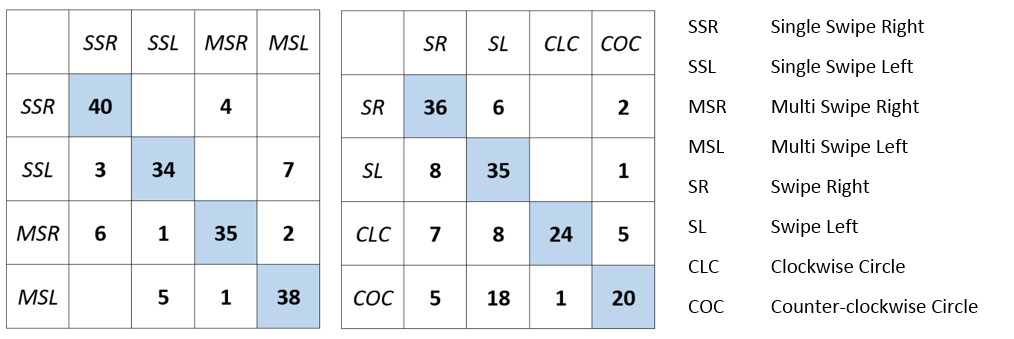
\includegraphics[width=0.8\textwidth]{images/armrest_eval_confustion}
\captionof{figure}{Confusion matrices of recognized gestures for touch interaction (left) and free-air interaction (right)}
\label{fig:armrest_eval_confustion}
\end{minipage}

We performed a study with 11 participants investigating three different aspects - the detection rate of the gesture recognition system, differences in interaction speed between the two methods and getting a general feedback on the usability of our system. After a short introduction the participants were asked to perform each gesture 4 times for both sets in alternating starting order. The results are shown in Figure \ref{fig:armrest_eval_confustion}. The touch interaction performed reasonably with a detection rate between $79.5\%$ and $90.9\%$ for each gesture. The detection rates of the free-air interaction were considerably lower, ranging from $45.5\%$ for counter-clockwise circles to $81.8\%$ for swipes to the right. The main issue is distinguishing between single and multi-touches. A personalized threshold that is calibrated to the user might alleviate this issue in future iterations. The interaction zone above the finger area is limited to a range of about 15 cm. While performing the circular gestures the participants often left this area, leading to misattribution to swipe gestures.

In the second part of the evaluation the participants had to perform a task in the presented demonstration application - selecting and playing back a certain music file. We calculated the time required to perform the task. The average time for free-air gestures ($\mu=125.67s, \sigma=95.12s$) was considerably higher than the average task completion time for touch gestures ($\mu=34.26s, \sigma=28.61s$). It is noticeable that there is a very high deviation of the different runs, while the touch gestures fare better in general. While many users were able to quickly perform the task, others had a high number of errors and required several minutes. We can assume that a certain amount of training can reduce the required time. A trained user not participating in the study required 11 s for the touch gestures and 18 s for the free air gestures.

Finally, we asked the participants to fill a general questionnaire on their experience with the Active Armrest comprised of a number of Likert-scale (1-10) questions. There was a strong preference for the touch gestures, in line with the results of the interaction time and gesture recognition study (1=touch gestures, $\mu=1.72, \sigma=0.84$). Most participants could imagine using the system for a longer period of time in their cars (10=strong agree, $\mu=8.00, \sigma=2.00$) and considered the device intuitive to use (10=strong agree, $\mu=8.36, \sigma=1.67$) and is an interesting interaction device (10=strong agree, $\mu=8.63, \sigma=1.26$). The touch interaction pattern was considered easier to use (10=very easy, $\mu=8.00, \sigma=2.45$) than the free-air interaction (10=very easy, $\mu=3.64, \sigma=2.68$). The opinions on the device precision were mixed (10=very precise $\mu=7.27, \sigma=2.43$).

